\documentclass[letterpaper,twocolumn,10pt]{article}
\usepackage{usenix,epsfig,endnotes}
\usepackage{float}
\usepackage{subfigure}
\usepackage{algorithm} %format of the algorithm
\usepackage{algorithmic} %format of the algorithm
\usepackage{multirow} %multirow for format of table
\usepackage{amsmath}
\usepackage{xcolor}
\usepackage{url}
\usepackage{hyperref}
\usepackage{breakurl}
\usepackage{xspace}
 \usepackage{flushend}
%\usepackage{Utopia}

\renewcommand{\algorithmicrequire}{\textbf{Input:}}
\renewcommand{\algorithmicensure}{\textbf{Output:}}



\newcommand\LSMForest{{LSM-Forest}\xspace}
\hyphenation{LSM-Forest}

\newcommand\DBC{Distributed BloomCluster\xspace}
\newcommand\DBCs{DBC\xspace}
\newcommand\DBCss{DBCs\xspace}


\begin{document}

%don't want date printed
\date{}


\title{Title}

\author{

} % end author

\maketitle 
\subsection{Impact of Simple Scheduling Strategies}
\label{sec3.2-0}

In this section, we introduce a simple segment-based
balancing method based on historical records and 
greedy strategy, which move segments periodically to 
rebalance the throughput of block servers.
Moreover, the influence of different parameters on
the scheduling results will be analyzed.

\subsubsection{Introduction to Simple Scheduling 
Strategies} \label{sec3.2-1}

In order to analyse if the scheduling strategy is good, 
we need to define an index to measure the level of load
balance. Here we choose the variance of read throughput
between block servers as a measurement. As the variance
changes over time, we use median of variances over time
as a measurement when we want to judge the schedule
effect over a period of time. Due to the fact that the
movement of a segment employs computation resource as
well as time, we define the number of moving as the 
schedule cost. Thus, the target of rebalance is to
minimize read throughput and schedule cost.

We first define a simple greedy strategy, which 
performs a round of schedule at a specified time
interval (to be specified by the administrator).
When the time to schedule arrives, the scheduler 
will calculate the historical average on every 
segment over a period of time. Then, the scheduler 
will traverse segments by historical records from
high to low. The scheduler will move the segment to
the block server which has the lowest throughput.
Obviously, schedule frequency and the time length of 
historical record will make an impact on the schedule 
result.

According to the 80/20 rule, we have a reason to believe
that few segments contributes most to the variance of the
entire cluster. Hence, we define a \textit{partial greedy
strategy}, which only replace segments with the most
throughput in each round of schedule. Evidently, the
proportion of segments to schedule each time will also make
an impact on the schedule result.

\subsubsection{Upper Bound of Algorithm}\label{sec3.2-2}

Scheduling effect not only depends on strategy itself, but
also depends on the schedulability of the cluster. We use
the following method to attempt to reach an approximate
upper schedule bound of a cluster. In the simple greedy
strategy, we pretend to know the future throughput of each
segment, and execute scheduling with the future throughput.
Besides, schedule should be frequent enough. We use trace
of clusters in business environment for simulation.

\begin{table}[]
    \centering
    \begin{tabular}{c|c|c|c|c}
         Cluster & Type & No Schedule & Upper Bound & Greedy\\
         AY306L & ESSD & 2.13E+18 & 5.36E+17 & 6.51E+17\\
         AY251Z & ESSD & 7.68E+17 & 1.99E+17& 5.53E+17\\
         AY272T & SSD & 6.87E+17 & 3.02E+06 & 1.10E+17\\
         AY306O & Efficient & 3.08E+17 & 3.29E+06 & 1.14E+17\\
         AY336D & Efficient & 7.27E+17 & 3.35E+06 & 1.12E+17\\
         AY272M & Efficient & 2.97E+17 & 3.52E+06 & 7.75E+16\\
    \end{tabular}
    \caption{Median of cluster variance}
    \label{table3.2-1}
\end{table}

Table \ref{table3.2-1} shows the initial state and the
approximate upper bound of any algorithm. Note that, there
is little potential for ESSD clusters to improve, while SSD
clusters and efficient clusters have great potential to
improve. As was stated in section \ref{sec3.2-1}, ESSD
cloud disks have better performance and allow higher
throughput. Thus, user are more likely to read and write
more to the disk and the smallest unit of scheduling will
be larger. This makes scheduling algorithm less effective
on clusters with higher performance.

\subsubsection{Effect of Greedy Algorithm}\label{sec3.2-3}

We simulate simple greedy algorithm on different clusters.
We can find that simple greedy strategy can reduce the
variance in some degree, but there's still some distance
to the upper limit(Table \ref{table3.2-1}). What's worse,
sometimes, negative optimizations may occur(Figure
\ref{fig3.2-1}). The reason is that average of historical 
records can not describe the pattern of the cluster
properly. 

\begin{figure}[h]
    \centering
    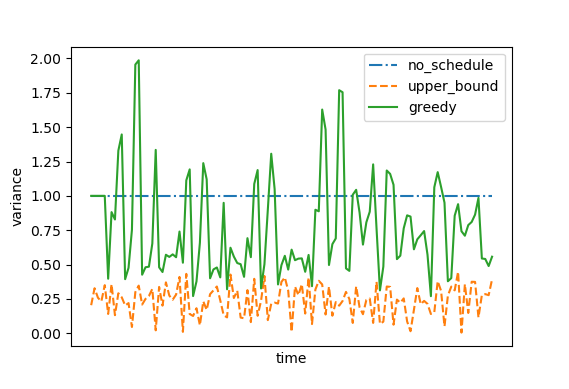
\includegraphics[width=0.4\textwidth]{Figure-3.2/Figure_1.png}
    \caption{Result of Simple Greedy Strategy on AY251Z}
    \label{fig3.2-1}
\end{figure}

For example, I/O pattern of many segments is periodic. In
cluster AY251Z, the I/O pattern of a device, which has 16
segments and accounts for 9.2\% flow of the whole cluster,
is in a cycle of 20 minutes. However, Figure \ref{fig3.2-2}
indicates that these segments are in busy only in a short period of the cycle. If the observation range of history is
too low, prediction will differ greatly from the actual
state. However, if we raise the observation range, in some
segments, local characteristics will be missed, though the
periodic problem may be solved. As a result, detailed I/O
pattern should be extracted for scheduling.
\begin{figure}[h]
    \centering
    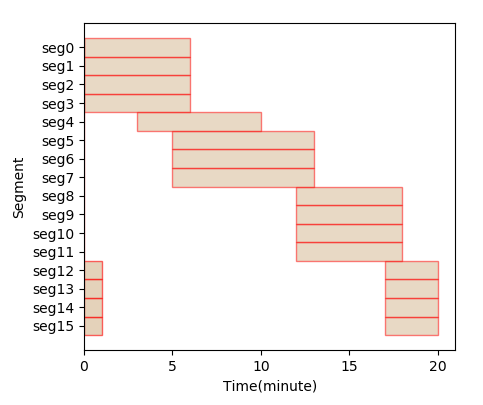
\includegraphics[width=0.4\textwidth]{Figure-3.2/Figure_2.png}
    \caption{Busy Time of Segments in a Certain Device}
    \label{fig3.2-2}
\end{figure}

\subsubsection{The Proportion of Segments to Schedule}\label{sec3.2-4}

As was stated in section \ref{sec3.2-1}, the proportion
of segments to schedule each time will make an impact on
the schedule result. Figure \ref{fig3.2-3} shows the
relation between variance and the schedule proportion of \textit{partial greedy strategy}. Schedule interval and
observation length of history are both 5 minutes.

\begin{figure}[h]
    \centering
    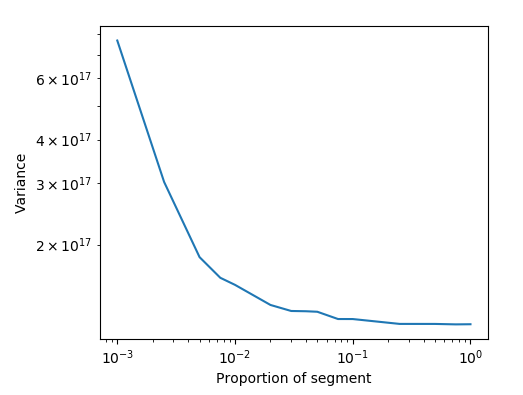
\includegraphics[width=0.4\textwidth]{Figure-3.2/Figure_3.png}
    \caption{Variance of Cluster with Different Schedule  Proportion}
    \label{fig3.2-3}
\end{figure}
From the figure, we can learn that from the point of view 
of results, there is no significant difference between
implementing greedy schedule for all the segments and for 
only 10\% of all segments. Few segments contributes most to
the variance.




% Use shows the following at camera-ready time to suppress page numbers.
% Comment it out when you first submit the paper for review.
%\thispagestyle{empty}



\bibliographystyle{acm}
\bibliography{references}


\end{document}
